\chapter{Thermodynamics}
\section{Kinetic theory}
If KE is dependent on temperature, whats the difference between a cold moving ball, and a hot stationary ball. This is because the former is about \textbf{microscopic}, but the latter is about \textbf{macroscopic}. 

Because it is not feasible to model the motion of every single molecules with newton's laws, it is more convenient to use probability.

\subsection{Probability distribution}
We are working with \textbf{continuous} probability distribution $P(x) $where $0 \leq P(x) \leq 1$. The area under the curve (let's say from $a$ to $b$, $b>a$) would be the probability of the number $n$ to be $a\leq n\leq b$

\subsection{velocity distribution}
let the velocity probability distribution be $g(v_x)$
\begin{equation}
    g(v_x)\propto \exp\bigg({\frac{-mv_x^2}{2k_B T}}\bigg)
\end{equation}

To find the proportionality constant, we have to normalise the distribution by integrating the distribution from -1 to 1, and setting the integral to 1.

\begin{equation}
    \int_{-\infty}^{\infty}A\exp\bigg({\frac{-mv_x^2}{2k_B T}}\bigg)dv_x = 1
\end{equation}
This is the case where $\alpha=m/2k_BT$ (see Math section). Hence,
\begin{equation}
    g(v_x)=\sqrt{\frac{m}{2\pi k_B T}}\exp\bigg({\frac{-mv_x^2}{2k_BT}}\bigg)
\end{equation} 

To find the average velocity, we just need to integrate 
\begin{equation}
    \langle v_x \rangle =\int_{-\infty}^{\infty}v_xg(v_x)dv_x=0
\end{equation}
HAHA sike it is 0 cos its velocity not speed.

\subsection{speed distribution}
Speed $v=\sqrt{v_x^2+v_y^2+v_z^2}$ can be represented as the distance between the origin and a point in the velocity space.
\begin{figure}[H]
    \centering
    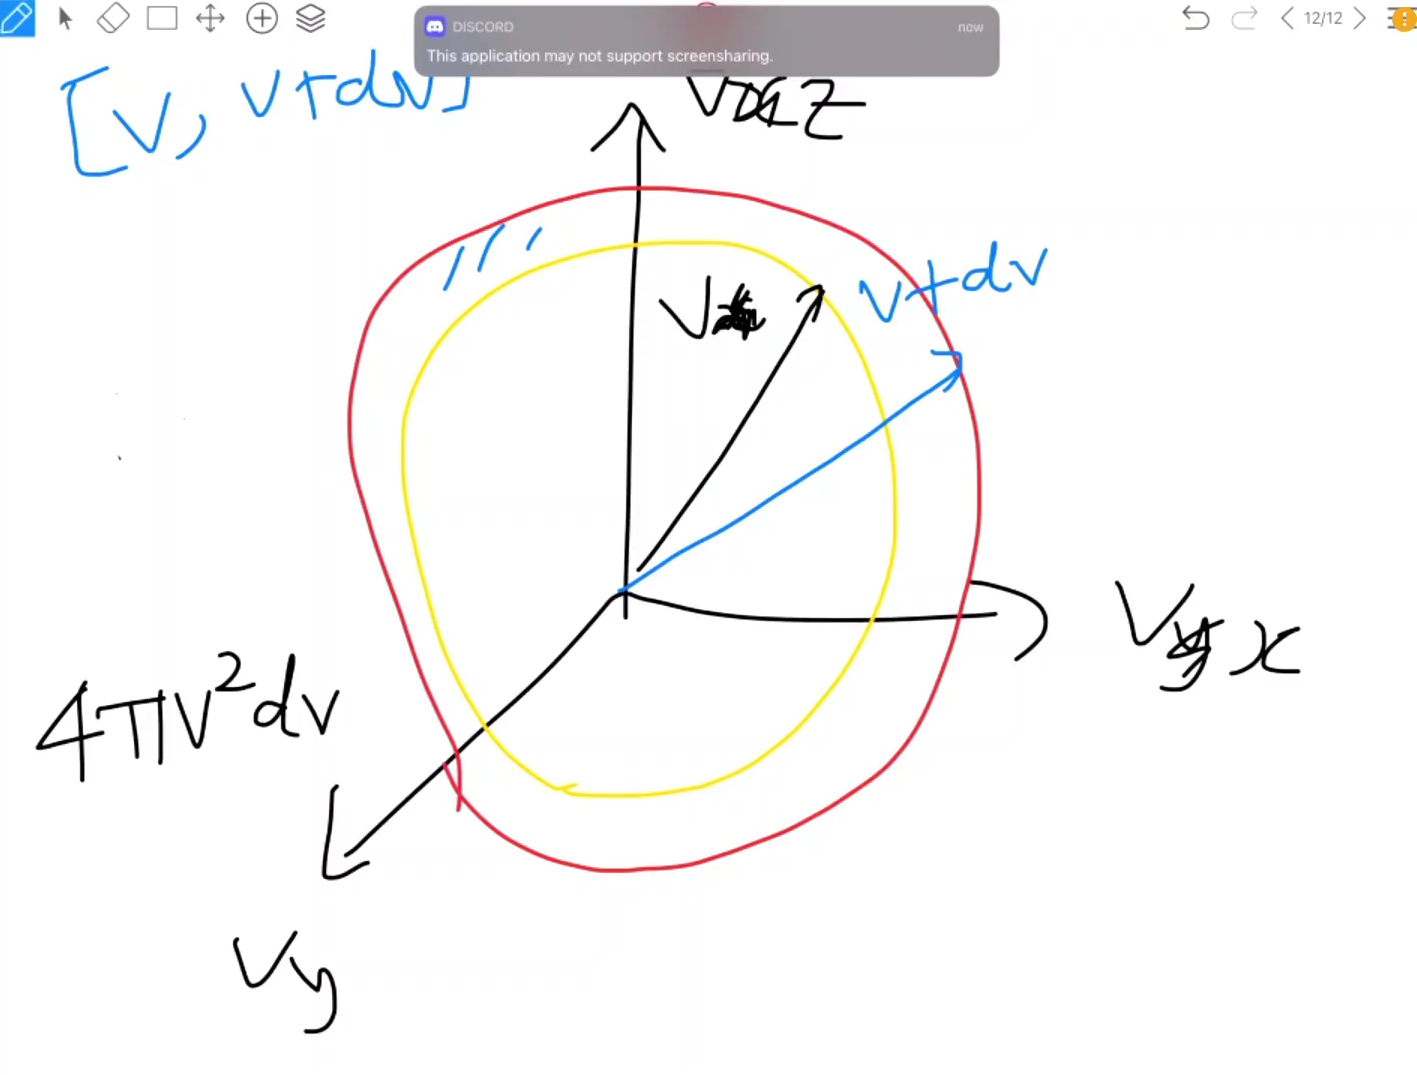
\includegraphics[width=0.5\linewidth]{velocity space.png}
    \caption{beautiful drawing by Ryan}
    \label{<label>}
\end{figure}
The volume enclosed, $V=4\pi v^2 dv$, between the red and yellow circle, multipled by the probability of the particles moving in that region, denotes the particles with speed $v \leq v_p \leq v+dv$. The speed probability distribution is then given by
\begin{equation}
    f(v)dv\propto v^2 \exp \bigg({\frac{-mv^2}{2k_B T}}\bigg)dv
\end{equation}

Integrating, we get
\begin{equation}
    f(v)=\frac{4}{\sqrt{\pi}}\bigg(\frac{m}{2 k_B T}\bigg)^\frac{3}{2} v^2 \exp\bigg({\frac{-mv^2}{2k_BT}}\bigg)
\end{equation}

Average speed:
\begin{equation}
    \langle v \rangle =\sqrt{\frac{8k_BT}{\pi m}}
\end{equation}

Root mean squared velocity: 
\begin{equation}
    \langle v^2 \rangle =\frac{3k_BT}{m} = \langle v_x^2\rangle + \langle v_y^2\rangle + \langle v_z^2\rangle
\end{equation}

Most probable speed: $df/dv=0$
\begin{equation} 
    v=\sqrt{\frac{2k_BT}{m}}
\end{equation}

Note: $m$ stand for the \textbf{molar mass} lmao not the actual mass of all the gas molecules. 

\subsection{Equipartition theorem}
Every degree of freedom will contribute $k_B T/2$ to the internal energy. 
\begin{equation}
    U=\frac{f}{2}k_BT
\end{equation}

More rigorous form: Each quadratic mode with energy in the form of $E=\alpha x^2$, where $x$ can be position or velocity, contributes $k_BT/2$ to the internal energy (so its not really about degree of freedom). It just so happens that both rotational and translational energy are $\propto v^2, \omega^2$

\subsection{Ideal gas law}
\begin{equation}
    p=\frac{1}{3}n m \langle v^2 \rangle
\end{equation}
where $n$ is the number of molecules per unit volume. and $m$ is the mass of the molecules.

\section{How molecules move}
\subsection{Solid Angle}
In 2D, we have $s=r\theta$. In 3D, $A=r^2 \Omega$, where $\Omega$ is the solid angle (imagine the tip of the cone), and $A$ is the curved surface at the base of the cone. $\Omega \in [0,4\pi]$, as the maximum area subtended by a solid angle is that of a sphere: $A=4\pi r^2$

It is the same as if we have some angle $\theta$, and we increase by $d\theta$, the change in area on the spherical surface with unit length $1$ is $dA= 2\pi \sin \theta d\theta$. If we calculate with solid angle instead, where $\Omega \to \Omega + d\Omega$, $dA=(\Omega + d\Omega)r^2-\Omega r^2 = r^2 d \Omega$.
Hence, we obtain the \textbf{conversion factor} between $\Omega$ and $\theta$
\begin{equation}
    d\Omega=2\pi \sin \theta d\theta
\end{equation}

Imagine a bunch of particle being yeeted out from a point in all direction, the proportion of particle passing through a spherical cap with solid angle $d\Omega$ is $d\Omega/4\pi = \sin \theta d\theta/2$

\textcolor{blue}{\textit{There is a wall with area $A$. In time $dt$, what is the number of molecules that hit the wall that have $v \in [v,v+dv]$ and $\theta \in [\theta,\theta+d\theta]$.}}
Let $\rho_n$ be the volume number density, the number of molecules (per unit volume) that satisfy the condition (ignoring the wall)
\begin{equation}
    \rho_n f(v)\bigg(\frac{1}{2}\sin\theta\bigg)\,dv\,d\theta
\end{equation}
The number of particles that will hit the wall with area $A$ in time $dt$ would be 

\begin{equation}
    \rho_n f(v)\bigg(\frac{1}{2}\sin\theta\bigg)\,dv\,d\theta (A v \,dt \cos \theta )
\end{equation}
To find the number of particles hitting the wall \textbf{per unit area} and \textbf{per unit time}, we let $A$ and $dt$ be 1 (which is abit scam). The change in momentum experienced by those particles would then be 
\begin{align}
    dp &= (2mv \cos \theta)  \rho_n f(v)\bigg(\frac{1}{2}\sin\theta\bigg)\,dv\,d\theta v \cos \theta \\
    \textsf{Pressure} &= \int_{0}^{\infty}\int_0^{\frac{\pi}{2}}dp 
\end{align}
From here, you can derive the ideal gas equation: $pV=nRT$

\subsection{Molecular flux}
Molecular flux is the number of molecules striking the unit area per unit time (second). To calculate this, we just
\begin{align}
    \int_{0}^{\infty}\int_0^{\frac{\pi}{2}} &=\rho_n f(v)\bigg(\frac{1}{2}\sin\theta\bigg)\,dv\,d\theta \,v \cos \theta\\
    \Phi &= \frac{1}{4}\rho_n \langle v \rangle
\end{align}
where molecular flux is usually denoted as $\Phi$. So if you have a box with a hole of area $A$ through which gas is allowed to escape, the number of molecules escaping per second would just be $N=\Phi A$. This process is called \textbf{Effusion}. Note that this formula only works if the area, $A$, is small. If $A$ is large, you will need to consider edge effects as the particles bouncing off some other surface can also escape through the hole. So, how small should the hole be? The condition is that 
\begin{equation}
    d \ll \lambda \, \textsf{, where $\lambda$ is the mean free path}
\end{equation}
The particle exiting from the small hole will \textbf{not} follow the Maxwell Boltzmann distribution becuase effusion is not a fair selection (if molecule is moving faster, it will have a higher chance of exiting the hole). 
\subsection{mean free path}
Mean free path is the average distance that a gas particle can travel before it collides with another particle. 

The mean collision time, $\tau$, is the average time that a gas particle takes to collide with another particle. We can define $\sigma$ as the cross-sectional area of the particle, and $P(t)$ as the probability of a particle \textbf{not} colliding up to a time $t$. 
\begin{align}
    P(t+dt)&=P(t)+\frac{dP}{dt}dt\\
    &= \underbrace{P(t)}_{\textsf{Probability of not colliding up till $t$}} \times \underbrace{(....)}_{\textsf{probability of not colliding in $dt$}}\\
\end{align} 
In time $dt$, the particle will sweep a volume of $v\sigma dt$, and we want no molecule to be inside this volume. The probability of having a molecule inside this volume is $\rho_n v \sigma dt$, hence
\begin{equation}
    P(t)+\frac{dP}{dt}dt=P(t)\times\underbrace{(1-\rho_n v\sigma dt)}_{\textsf{probability of not colliding in $dt$}}
\end{equation}
We can just solve the differential equation by separation of variable and get the probability of a molecule not colliding up to time $t$ as
\begin{equation}
    P(t)=\exp(-\rho_n \sigma v t)
\end{equation}
Probability that it collides in the next $dt$ is 
\begin{equation}
    \underbrace{(e^{-\rho_n \sigma v t})}_{\textsf{not colliding up till $t$}} \times \underbrace{\rho_n \sigma v dt}_{\textsf{colliding in $dt$}} 
\end{equation}
Averaging it out across all time,
\begin{align}
    \langle t \rangle &= \int_0^{\infty}t(e^{-\rho_n \sigma v t})(\rho_n \sigma v dt)\\
    \tau &= \frac{1}{\rho_n \sigma v}
\end{align}

Since $\lambda=\langle v\rangle \tau = \langle v_r \rangle/\rho_n \sigma v$ where $v_r$ is the relative speed. And according to maxwell boltzmann disribution, $\langle v \rangle \approx \sqrt {\langle v_r ^2 \rangle} \approx \sqrt{2} \langle v \rangle$

\section{First Law of thermodynamics}
The first law of thermodynamics state that:
\begin{equation}
    \Delta E= \Delta Q + W
\end{equation}
Since there is a plus sign in front of $W$, it must mean \textbf{work done on the gas}.
The differntial form of the the equation above is
\begin{equation}
    dE=dQ+dW
\end{equation}
where $dQ$ and $dW$ are called \textbf{inexact differential} since they are path dependent (and not state dependent)quantities.

On the other hand, $E$ is a state dependent quantity (depends on both temperature, $T$ and volume, $V$). Hence, a small change in $E$ ($dE$) can also be written as
\begin{equation}
    dE(T,V)=\bigg(\frac{\partial E}{\partial T}\bigg)_V dT+\bigg(\frac{\partial E}{\partial V}\bigg)_T dV
\end{equation}
\begin{mybox}{gray}{Molar specific heat at constant \textbf{volume} and \textbf{pressure}}
    Molar specific heat:
    \begin{itemize}
        \item at constant \textbf{volume}
              \begin{equation}
                  C_V=\bigg(\frac{\partial Q}{\partial T}\bigg)_V=\bigg(\frac{\partial E}{\partial T}\bigg)_V
              \end{equation}
              Proportionality factor between heat supplied and temperature change of a system at constant volume
        \item at constant \textbf{pressure}
              \begin{equation}
                  C_p
                  =\bigg(\frac{\partial Q}{\partial T}\bigg)_p
                  =\bigg(\frac{\partial (E-W)}{\partial T}\bigg)_p
                  =\bigg(\frac{\partial E}{\partial T}\bigg)_p+
                  p\bigg(\frac{\partial V}{\partial T}\bigg)_p
              \end{equation}
    \end{itemize}
    (the plus sign in front of the work is because $dQ=dE-dW$, and $dW=-pdV$. This is before when volume of gas decreases, work must be done \textbf{on} it, increasing its internal energy).
    \begin{flushleft}
        Since $\big(\frac{\partial V}{\partial T}\big)$ at constant pressure is essentially $\frac{nR}{p}$, the second term reduces to just $nR$.
    \end{flushleft}

    $$\boxed{\therefore C_p=C_V+nR}$$
    This shows that it takes more heat to increase temperature for an isobaric process. This is because extra energy is needed to offset those used when the gas does work by expanding.

    This relationship can actually be derived through many other methods as well. But just need to remember
    \textbf{first law of thermodynamics}, \textbf{internal energy's dependence on both temperature and volume}, as well as the fact that \textbf{heat capacity is a proportionality factor between heat input and change in temperature (internal energy)}, then shld be okay :)

\end{mybox}
\subsection{Quasi-static process}
\textbf{Definition}: A thermodynamic process that happens slowly enough for the system to remain in internal \textbf{thermodynamic equilibrium} (no tendency for the state of a system to change spontaneously).or in Ryan's words: a smooth curve on the $p-V$ diagram.
\subsubsection{Assuming a quasi-static process}
I think for most questions that talk about isochoric, isothermal and isobaric processes, the process is assumed to be quasi-static. This is because to be isothermal, isochoric or isobaric throughout the processes, you must be able to state the temperature, pressure and volume of the system at each step, which is possible only if the system is in equilibrium continuously.

\subsubsection{If process is not quasistatic}

If the question is about adiathermal process (according to Blundell, if the process is both adiathermal [without the flow of heat] and reversible, it's called adiabatic), the process can be carried out both quasi-statically and non quasi-statically. If the process is not quasi-static , we can no longer use the equation for various thermodynamic processes to solve the question. However, it is still possible to solve such questions using \textbf{conservation of energy.}

\begin{mybox}{green}{Quasi-static (reversible) process (my own interpretation)}
    If a gas changes state from A to B, it is only quasi-static if the intermediate states are all in thermodynamic equilibrium. Work done by isothermal / isochoric / isobaric processes are calculated with the assumption that processes are quasi-static (because infinitely small increments of change represent a continuous function).

    \begin{flushleft}
        E.g. If the process involves adding or removing weights from a piston (with gas beneath it), and the piston settles into a new equilibrium position, such a process is not quasi-static because the temperature / pressure / volume of the intermediate state is unknown (not in equilibrium). (Or when the process happens too fast such that there's insufficient time for the gas to settle into equilibrium)
    \end{flushleft}

\end{mybox}

\section{Second law of thermodynamics}
\subsection{Statements and Principles}
\subsubsection{Statements}
\begin{itemize}
    \item \textbf{Clausius' statement}: No process is possible whose \textbf{sole result} is the transfer of heat from a \textbf{colder to hotter} body. 
    \item \textbf{Kelvin-Planck statement}: No process is possible whose sole result is the complete conversion of heat into work, $Q_{\textsf{in}}\neq W$.
\end{itemize}

\subsubsection{Carnot Prciniple}
\begin{itemize}
    \item An irreversible heat engine is less efficient than a reversible one. \footnote{Proven by connecting a irreversible heat engine to a reversible one, and assuming it is more efficient. This will lead to a heat transfer from the cold reservoir to the hot reservoir, which violates Clausius' Statement.}
    \item Efficiencies of all reversible heat engines between identical heat reservoirs are the same. \footnote{Connect two reversible heat engines, A and B working in opposite directions. If A transfers from hot to cold and B transfers the other way, you will find that $\eta_A \leq \eta_B$. Swapping them will give $\eta_B \leq \eta_A$. We can conclude that $\eta_A=\eta_B$.}
\end{itemize}

\subsection{Conditions for reversibility}
\begin{itemize}
    \item Frictionless/Quasistatic
    \item Engine must have same temperature as reservoir.\footnote{Proven by connecting 2 reversible heat engines. The hot reservoir will gain net heat of $Q_H-Q_H=0$, same applies to the cold reservoir. By $0^{\textsf{th}}$ law of thermodynamics, they must be at the same temperature since there is no net heat transfer.} (Limit it to isothermal processes when exchanging heat, and adiabatic when not.)
\end{itemize}

Any reversible cycle working between 2 constant temperature heat reservoir should have the same efficiency as the \textbf{carnot engine}.

\subsection{Clausius Inequality}
\begin{mybox}{gray}{Clausius' inequality}
    Clausius' inequality states that for any closed loop,
    \begin{equation}
        \oint \frac{dQ}{T} \leq 0
    \end{equation}
    and equality must hold for reversible reactions.
    If the close loop consists of an irreversible, and an reversible part, we can write 
    \begin{equation}
        \int_A^B \frac{dQ}{T} + \int_B^A\underbrace{ \frac{dQ_{\textsf{rev}}}{T}}_{dS} \leq 0
    \end{equation}
    \begin{equation}
        dS\geq \frac{dQ}{T}
    \end{equation}
    In a thermally isolated system, $dQ=0$, and you will arrive at the second law of thermal dynamics: 
    \begin{equation}
        \boxed{dS\geq 0}
    \end{equation}
\end{mybox}

\subsection{Entropy}
Entropy is a state function (only dependent on initial and final states). For a \textbf{reversible process}, it is defined as such
\begin{equation}
    S(B)-S(A)=\Delta S= \int_A^B \frac{dQ_{\textsf{rev}}}{T}
\end{equation}

In general however,
\begin{equation}
    \Delta S \geq  \int_A^B \frac{dQ_{\textsf{irrev}}}{T}
\end{equation}

\textcolor{blue}{It is important to note that $\Delta S$ only depends on state, so it is the same regardless of whether the process is reversible or not.}

\subsubsection{Steps} {From this link: \href{https://www.physicsforums.com/insights/grandpa-chets-entropy-recipe/}{Entropy recipe}):
\begin{enumerate}
    \item Apply the First Law of Thermodynamics to the irreversible process to determine the final thermodynamic equilibrium state of the system
    \item Forget about the actual irreversible process, and focus instead exclusively on the initial and final thermodynamic equilibrium states.
    \item Devise a reversible path between the same two thermodynamic equilibrium states. This reversible path does not have to bear any resemblance whatsoever to the actual irreversible process path. \footnote{For example, even if the actual irreversible process is adiabatic, the reversible path you devise does not have to be adiabatic.  You can even separate various parts of the system from one another, and subject each of them to a different reversible path, as long as they all end up in their correct final states. Plus, there is an infinite number of reversible process paths that can take you from the initial state to the final state, and they will all give exactly the same value for the change in entropy.  So try to devise a path that is simple to work with (i.e., for which it is easy to apply step 3)}
    \item For the selected reversible path, evaluate the integral of $dQ/T$ from the initial state to the final state, where $aQ$ is the incremental amount of heat added to the system along the sequence of changes comprising the reversible path. ($\Delta S = \int dQ_\textsf{rev}/T$), where the subscript rev refers to the reversible path.
\end{enumerate}

\subsubsection{Entropy change of system with constant heat capacity, $C$}
\begin{equation}
    \Delta S = \int_{T_i}^{T_f} \frac{dQ}{T} =\int_{T_i}^{T_f} \frac{C dT}{T}= C\ln\bigg(\frac{T_f}{T_i}\bigg)
\end{equation}

\subsubsection{Expansion of ideal gas from $T_i, V_i \to T_f, V_f$}
\begin{equation}
    \begin{aligned}
        \Delta S = \int \frac{dQ}{T} =\int_{T_i}^{T_f} \frac{dU+pdV}{T} &= \int_{T_i}^{T_f} \frac{nC_V}{T} + \int_{V_i}^{V_f} \frac{nR}{V}dV \\
        &= nC_V \ln \bigg(\frac{T_f}{T_i}\bigg) + nR\ln \bigg(\frac{V_f}{V_i}\bigg)\\
    \end{aligned}
\end{equation}

\subsubsection{Joule Expansion}
This is equivalent to and isothermal Expansion from $V_i$ to $V_f$. 
\begin{equation}
    \Delta S = nR \ln \bigg(\frac{V_f}{V_i}\bigg)
\end{equation}

For an adiabatic process, $dQ=0$. Hence, there is no change in entropy for an adiabatic process (\textbf{isentropic})

\subsection{Fundamental Relations}

Going back to the first law of thermodynamics and let $dQ=TdS$ (only true for reversible reaction), we get
\begin{equation}
    dU=TdS-pdV
\end{equation}
All variables in this system are functions of state. $dS$ and $dV$ are extensive variables while $p$ and $T$ are intensive variables. If you scale up a sysem by 2 times, entropy and volume have to increase, while temperature and pressure can still remain the same.

\subsubsection{Spontaneity of process}
Let's say a system gains $dQ$ from environment, which has instantaneous temperature and pressure of $T_\textsf{ext}$ and $p_\textsf{ext}$,
\begin{equation}
    dS-\frac{dQ}{T_\textsf{ext}} \geq 0 \footnote{The LHS represents the entropy change of the universe(which is always positive), where $dS$ is the increase in entropy of the system. }
\end{equation}

Applying first law of thermodynamics, the following condition must be satisfied for process to be irreversible
\begin{equation}
    dQ=dU+p_\textsf{ext}dV+ T_\textsf{ext}dS \leq 0
\end{equation}
\begin{enumerate}
    \item \textcolor{blue}{Isolated system:} $dQ=0$, and $dS>0$ for spontaneous process.
    \item \textcolor{blue}{Solid:} $dV=0$, $dS=0$, and $dU<0$ for spontaneous process. 
    \item \textcolor{blue}{Constant $S$ and $p_\textsf{ext}$:} $dS=0$, $\Delta U + p_\textsf{ext} \Delta V=\Delta H <0$
    \item \textcolor{blue}{Constant $V$ and $T_\textsf{ext}$:} $dV=0$, $\Delta U - T_\textsf{ext} \Delta S=\Delta A <0$, where A is the \textbf{Helmholtz Free Energy}.
    \item \textcolor{blue}{Constant $p_\textsf{ext}$ and $T_{\textsf{ext}}$:} $\Delta (H-TS)=\Delta G<0$, where G is the \textbf{Gibbs Free Energy}.
\end{enumerate}

\section{Heat engines}
A Carnot engine (engine is defined as something that converts heat into work, 2 adiabats + 2 isotherms, cyclic process). We can prove by analysing each individual process that:
\begin{equation}
    \frac{Q_H}{Q_L}=\frac{T_H}{T_L}
\end{equation}

The analysis is as such: 

\begin{figure}[htbp]
    \centering
    \begin{tikzpicture}[
        > = latex,
        dot/.style = {draw,fill,circle,inner sep=1pt},
        arrow inside/.style = {postaction=decorate,decoration={markings,mark=at position .55 with \arrow{>}}}
        ]
        \draw[<->] (0,4.3) node[above] {$p$} |- (4.3,0) node[right] {$V$};
        \node[dot,label={above right:$A$}] (@1) at (0.5,4) {};
        \node[dot,label={right:$B$}] (@2) at (2.5,3) {};
        \node[dot,label={right:$C$}] (@3) at (4,1) {};
        \node[dot,label={below left:$D$}] (@4) at (1.5,2) {};
        \draw[arrow inside] (@1) to[looseness=.7,bend right=20] (@2);
        \draw[arrow inside] (@2) to[looseness=.7,bend right=20] (@3);
        \draw[arrow inside] (@3) to[looseness=.7,bend left=20] (@4);
        \draw[arrow inside] (@4) to[looseness=.7,bend left=20] (@1);
        \draw[dashed,thin] (0,4) node[left] {$p_A$} -- (0.5,4);
        \draw[dashed,thin] (0.5,0) node[below] {$V_A$} -- (0.5,4);
        \draw[red, fill=green, -{Triangle[width = 8pt, length = 7pt]}, line width = 3pt] (2.3, 3.5) node[above] {$Q_H$} -- (2.0, 2.7);
        \draw[blue, fill=green, -{Triangle[width = 8pt, length = 7pt]}, line width = 3pt] (2.3, 2) -- (2, 1.2) node[below] {$Q_L$};
    \end{tikzpicture}
    \caption{Carnot engine. $AB$ and $CD$ are isotherms, while $BC$ and $DA$ are adiabats. $AB$ is maintained at constant temperature $T_H$, while $CD$ is maintained at constant temperature $T_L$.}
    \label{carrot}
\end{figure}

\begin{enumerate}
    \item $\boxed{A\to B}$, $Q_H=nRT_H \ln(V_B/V_A)$
    \item $\boxed{B \to C}$, $T_H/T_L=(V_C/V_B)^{\gamma-1}$
    \item $\boxed{C \to D}$, $Q_L=-nRT_L \ln(V_D/V_C)$
    \item $\boxed{D \to A}$, $T_L / T_H=(V_A/V_D)^{\gamma-1}$
\end{enumerate}

Efficiency a carnot engine (turns heat into work) is defined as the ratio of work done to the heat input,

\begin{equation}
    \eta=\frac{W}{Q_H}=\frac{Q_H-Q_L}{Q_H}=1-\frac{T_L}{T_H}
\end{equation}. 

The reason why $W=Q_H-Q_L$ is because the process is cyclic and there is no change in internal energy.

\begin{flushleft}
    However, for a refrigerator (engine run in reverse), the efficiency is defined as a different way. It is instead
    \begin{equation}
        \eta=\frac{Q_L}{W}
    \end{equation}
    It makes sense because efficiency in this case means the amount of heat you can \textbf{remove} from a refrigerator when the engine does a certain amount of work. (similar for a heat pump, where the engine does work to pump heat instead of remove heat).
\end{flushleft}
